\chapter{Predicting Future Floods and their Potential Collateral Damage}

In this chapter, the association between rainfall rate and the flood occurrences will be discussed in a more detail. In order to do this, the rainfall rate will be compared with two different variables which represent how severe the flood occurrence is: the amount of sub-districts affected by floods and the number of people who are affected by floods.

\section{Rainfall Rate and the Sub-districts Affected by Floods}

From the previous chapter, it can be concluded that there is a positive correlation between rainfall rate and the sub-districts that are affected by floods. In Figure \ref{fig=corrrainsub.png}, the data points regarding the relationship between the rainfall rate and the amount of sub-districts that are affected by floods in any given rate is shown.\\

\begin{figure}
\begin{center}
\graphicspath{ {./Pict/} }
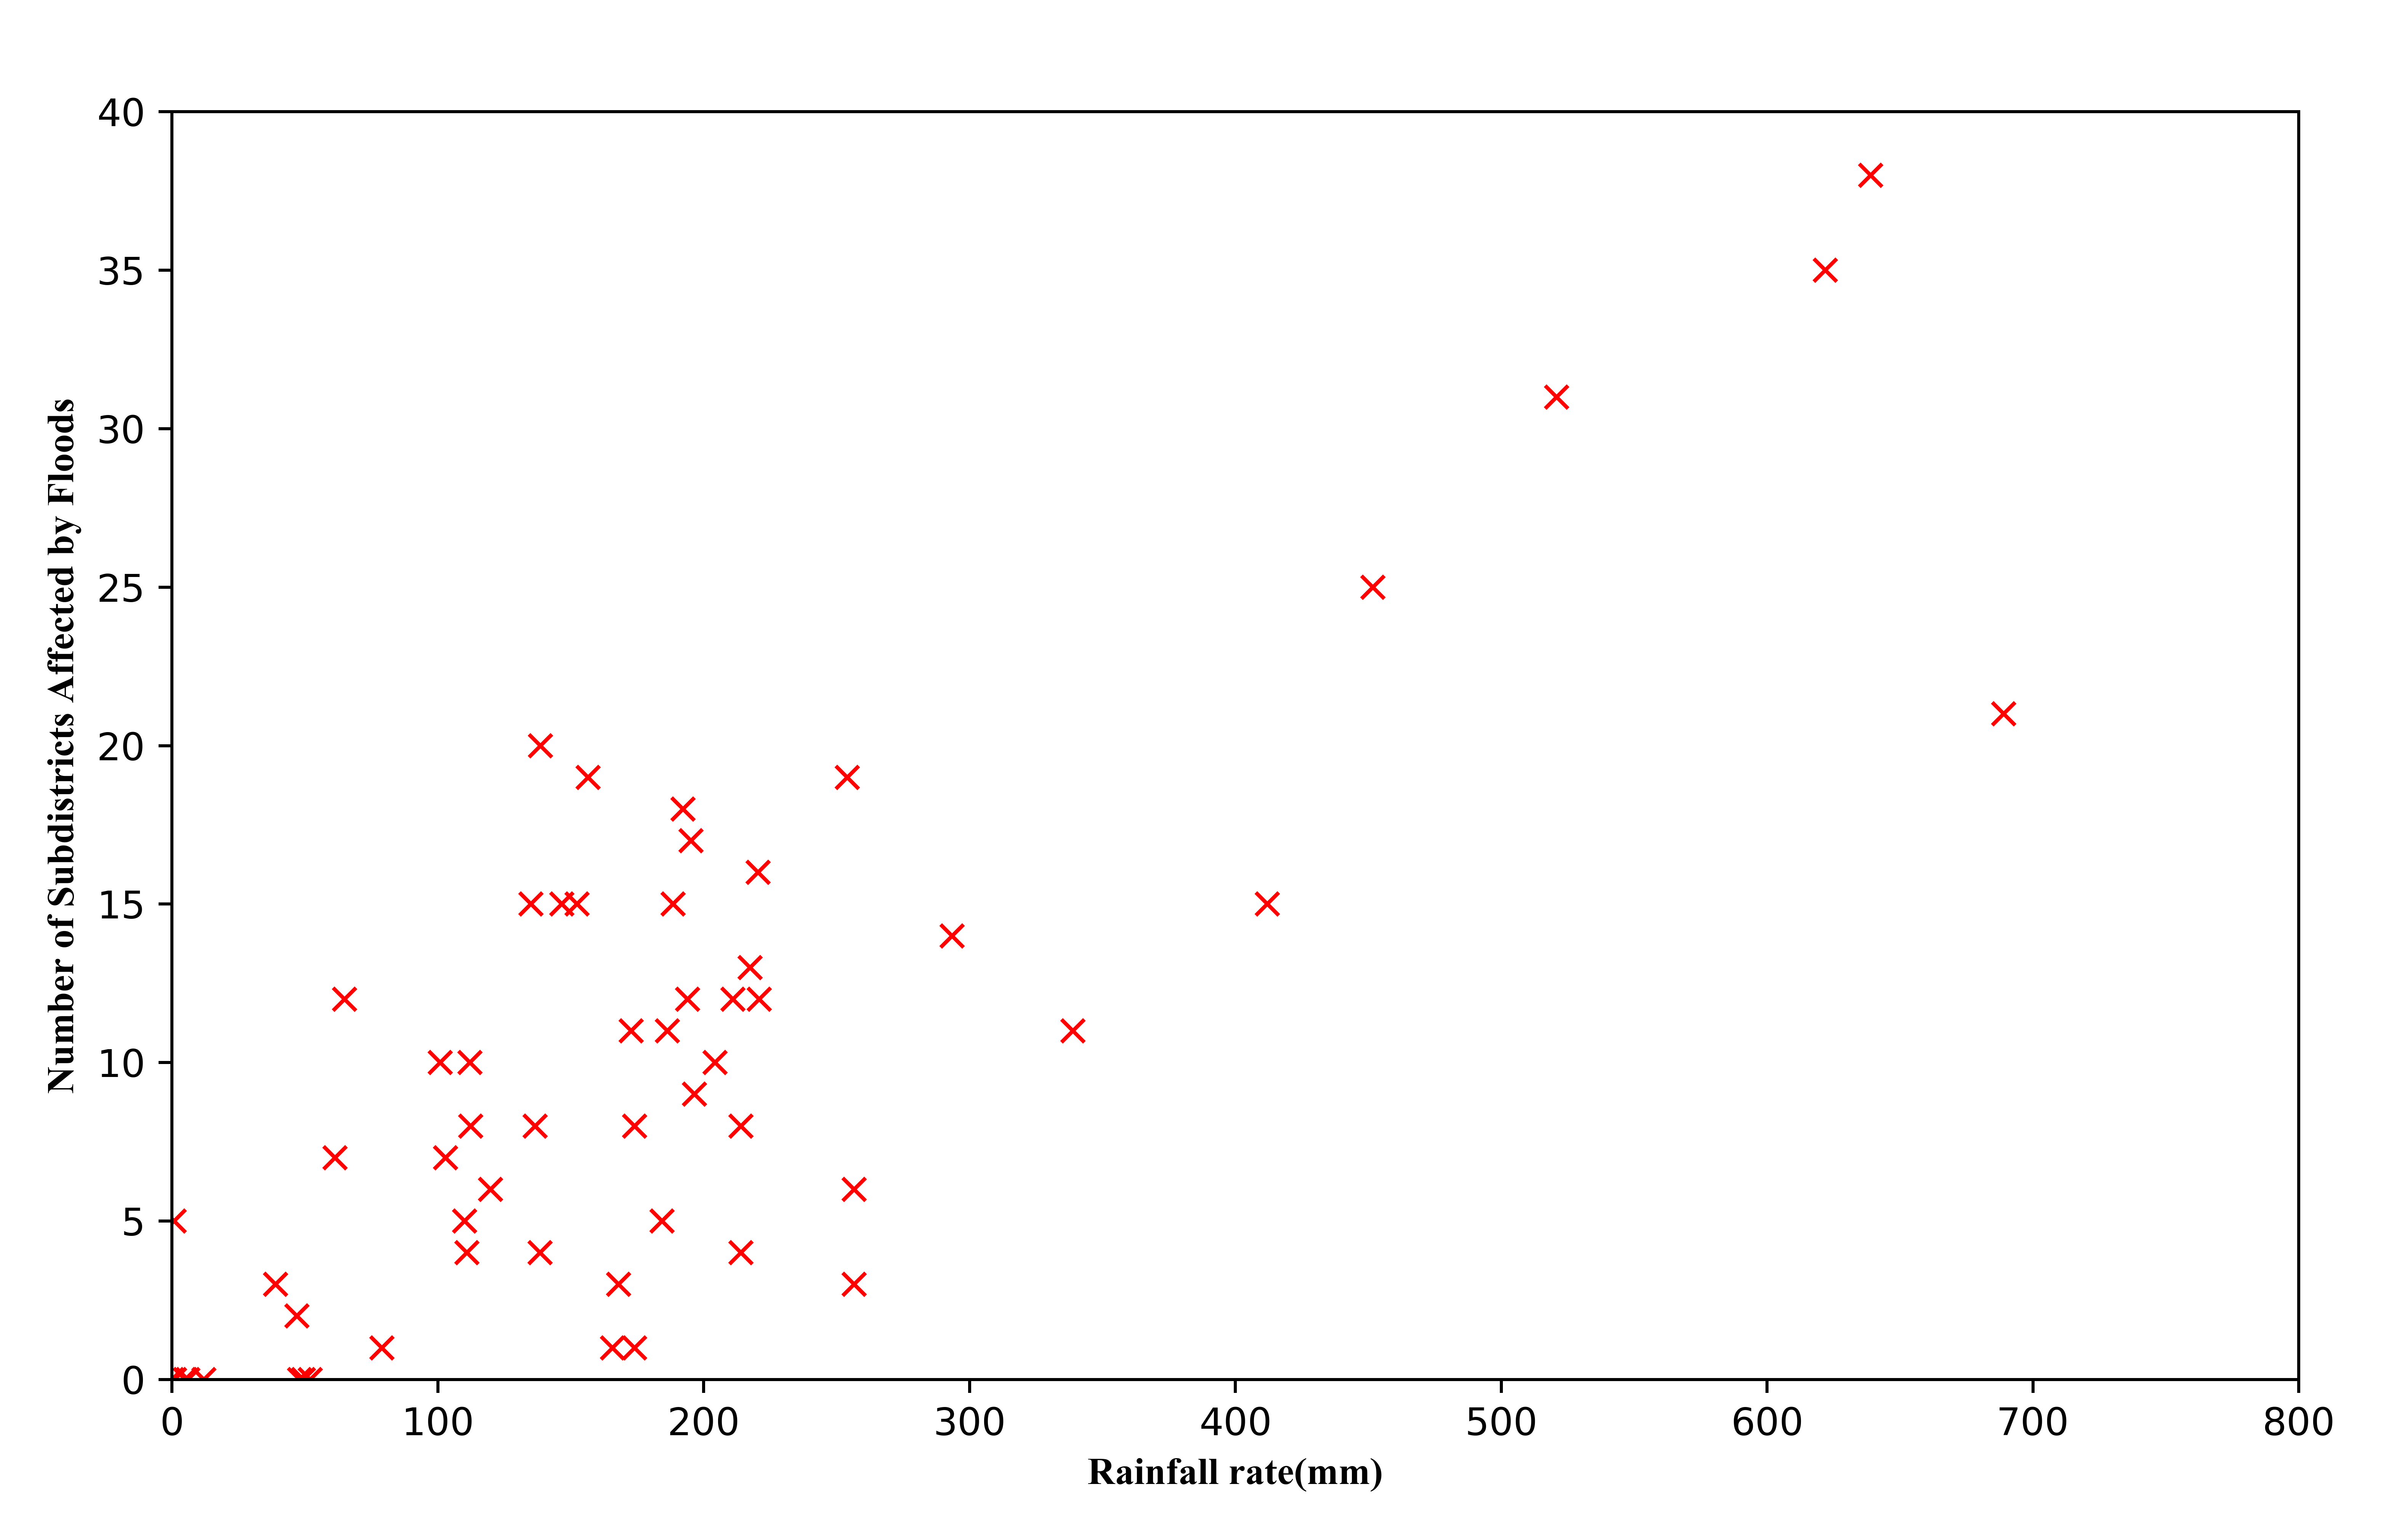
\includegraphics[scale=0.15]{corrrainsub.png}
\caption{Data points of rainfall rate and the sub-districts affected by floods}\label{fig=corrrainsub.png}
\end{center}
\end{figure}

\noindent
From Figure \ref{fig=corrrainsub.png}, it can be clearly seen that there is indeed a positive correlation between rainfall rate and the number of sub-district affected by floods. Also, by looking at the data points, a predictive modeling algorithm can be built. A linear regression model will be the appropriate modeling technique since the variance of the data points looks similar. Figure \ref{fig=corrrainsubreg.png} shows the linear regression model for this particular problem.\\

\begin{figure}
\begin{center}
\graphicspath{ {./Pict/} }
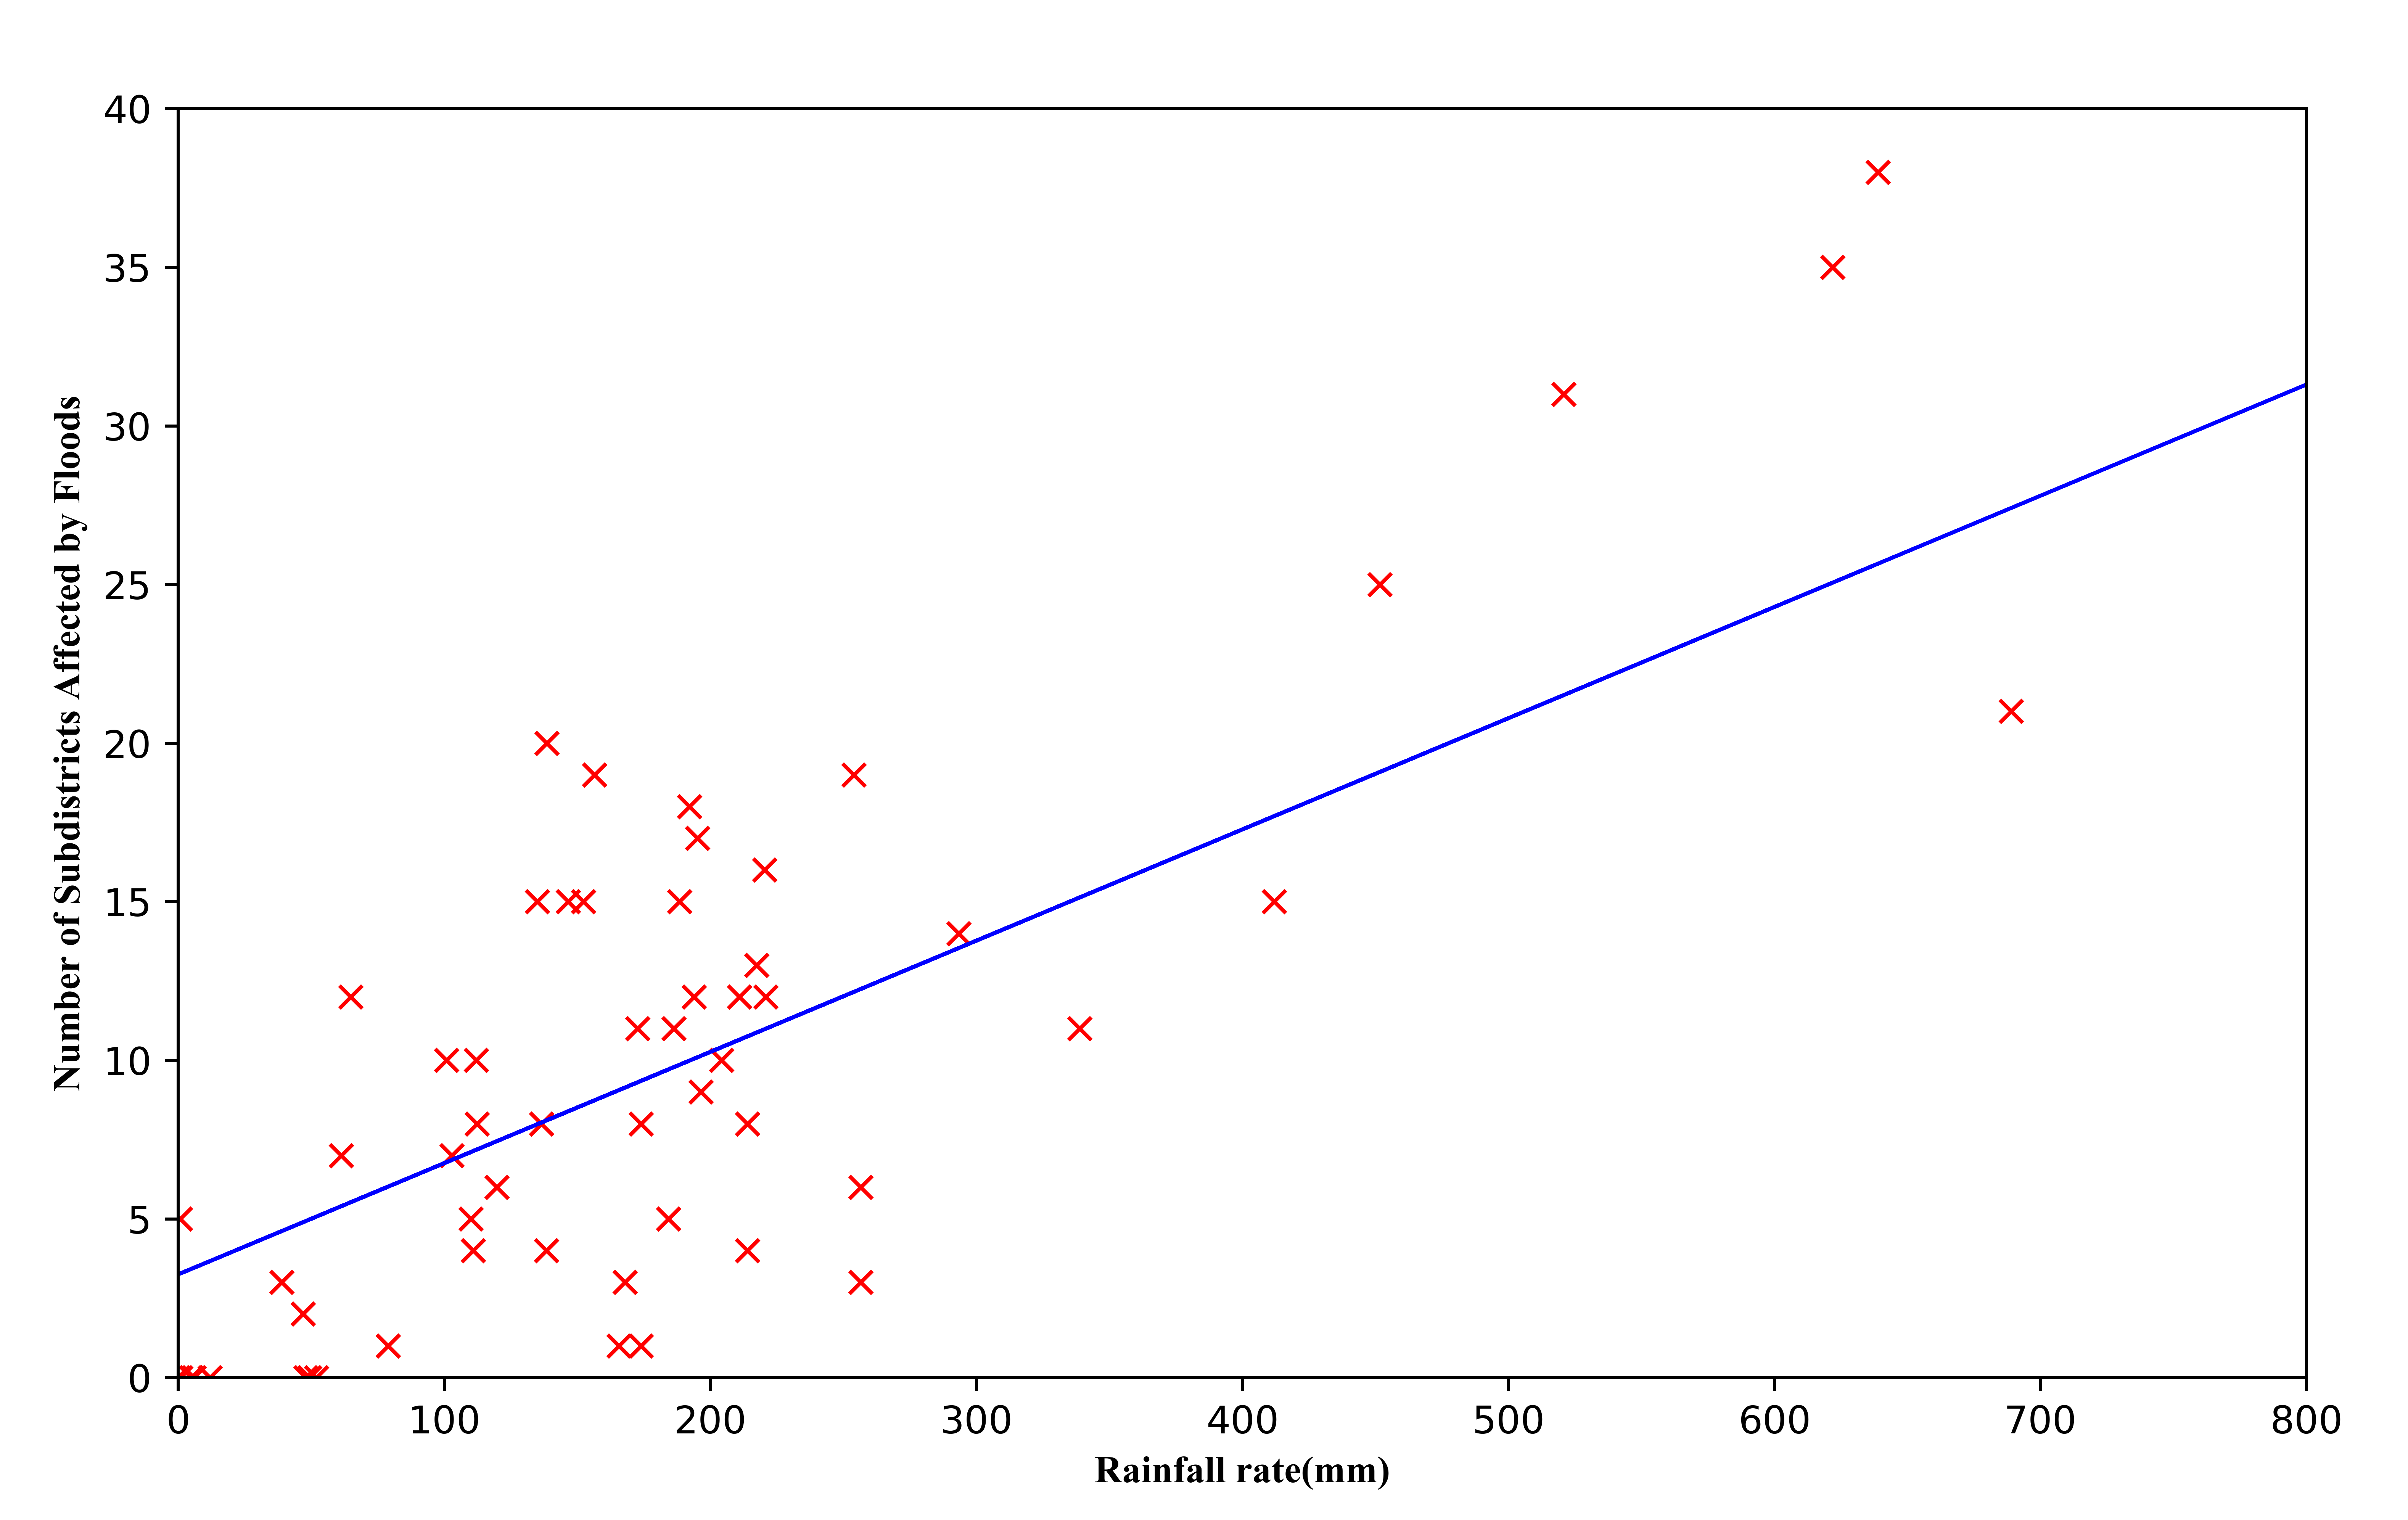
\includegraphics[scale=0.15]{corrrainsubreg.png}
\caption{Linear regression model to estimate the sub-districts affected by floods in any given rainfall rate}\label{fig=corrrainsubreg.png}
\end{center}
\end{figure}

\noindent
With the linear model, now the amount of sub-districts that will be affected by floods in any given rainfall rate can be estimated and prepared. The ability to predict the amount of sub-districts that will be affected by floods would be particularly important for the authorities to conduct some flood mitigation measurements in certain sub-districts.

\section{Rainfall Rate and the People Affected by Floods}
By now, it can be concluded that the amount of sub-districts that will be affected by floods can be estimated using a linear regression model. But how about the number of people who are affected by floods? To answer the question, similar steps as before will be conducted.\\

\noindent
Generally, one can assume that if the amount of sub-district affected by floods has a more or less linear correlation with the rainfall rate, then the same correlation applies for the number of people who are affected by floods. But does it? Figure \ref{fig=corrrainpeop.png} shows the correlation between two variables.\\

\begin{figure}
\begin{center}
\graphicspath{ {./Pict/} }
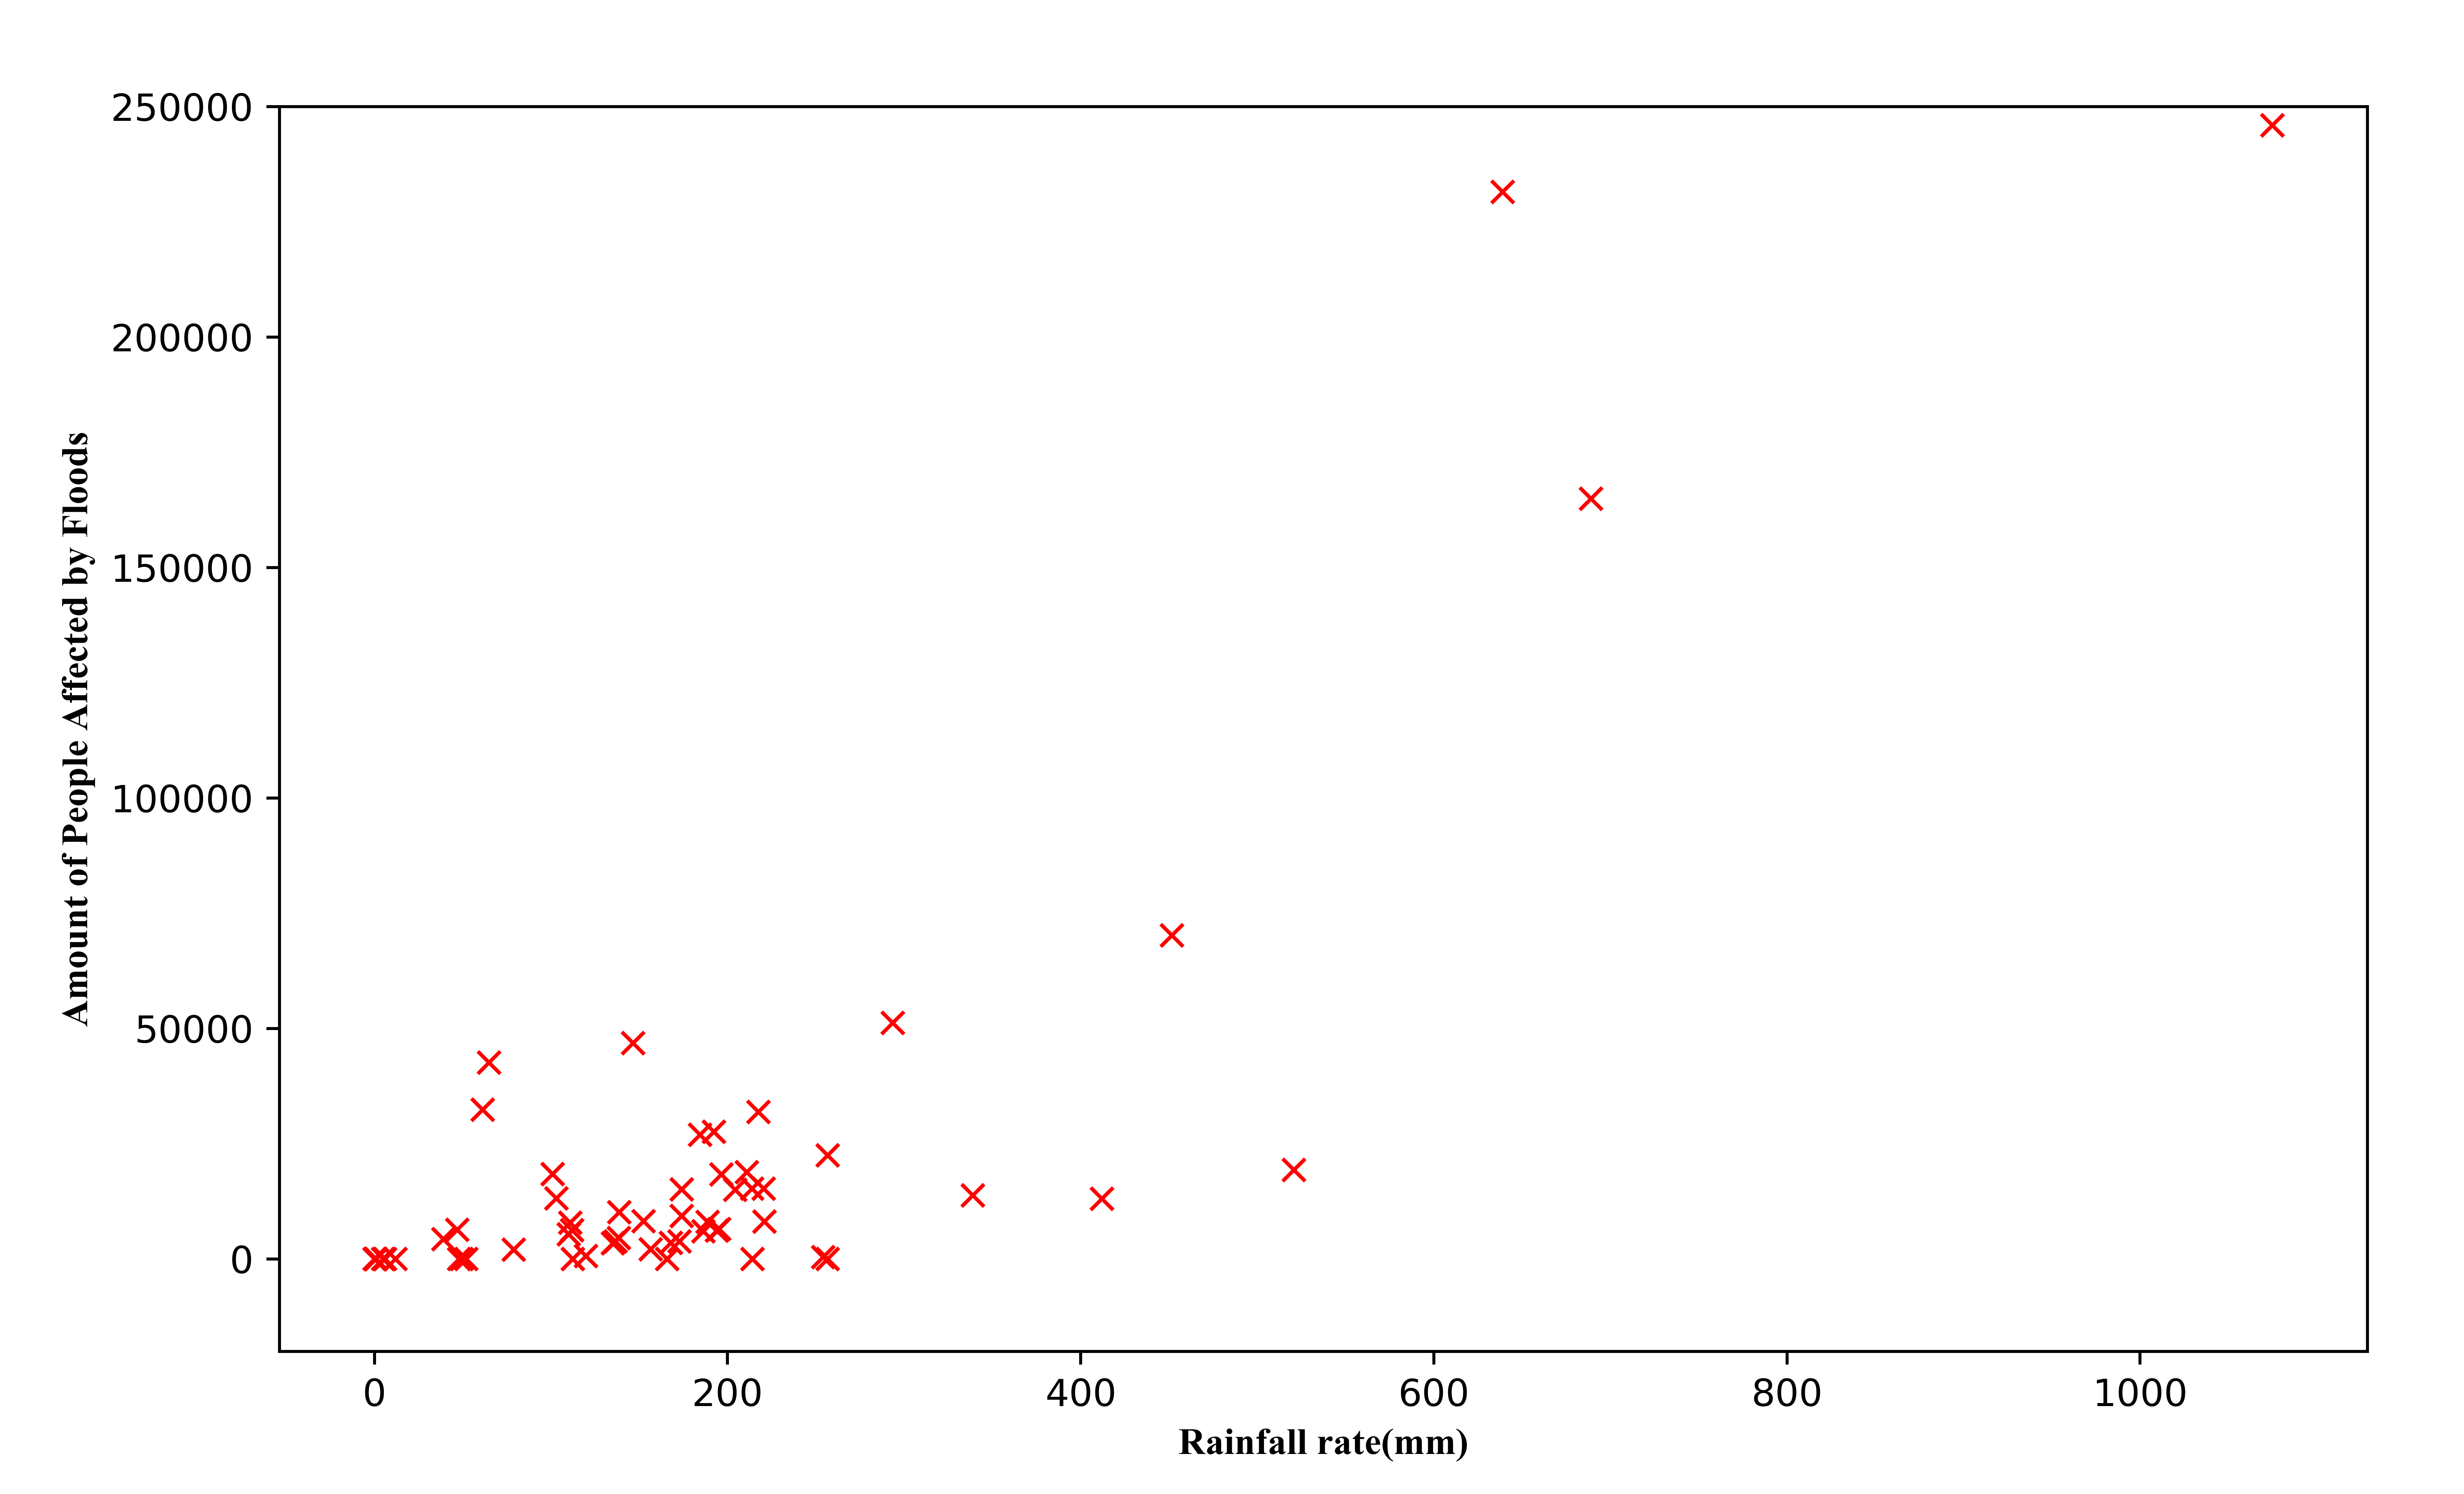
\includegraphics[scale=0.15]{corrrainpeop.png}
\caption{Data points of rainfall rate and the amount of people who will be affected by floods}\label{fig=corrrainpeop.png}
\end{center}
\end{figure}

\noindent
From Figure \ref{fig=corrrainpeop.png}, it can be concluded that rainfall rate also has a positive correlation with the amount of people who are affected by floods. However, by just looking at the data points, a linear model would not be an optimal model to predict the amount of people who are affected by floods because of the linearity characteristics wouldn't be able to catch the trend in the data points. Hence, a polynomial regression model will be more suitable for this particular problem.\\

\noindent
Before a polynomial regression model is applied, it is important to check which order that might be suitable for the problem. As an evaluation metric, R-squared or coefficient of determination is used. Figure \ref{fig=rsquare.png} shows how the R-squared score looks like when a polynomial regression model with variety of orders is applied within the test data of the data points in Figure \ref{fig=corrrainpeop.png}. As shown already, as the order of the polynomial model is higher than 4, the R-squared score is gradually decreasing. This phenomenon is a sign of overfitting since the model is trying to fit-in the data points which in turns give a high error and low number of R-squared.\\

\begin{figure}
\begin{center}
\graphicspath{ {./Pict/} }
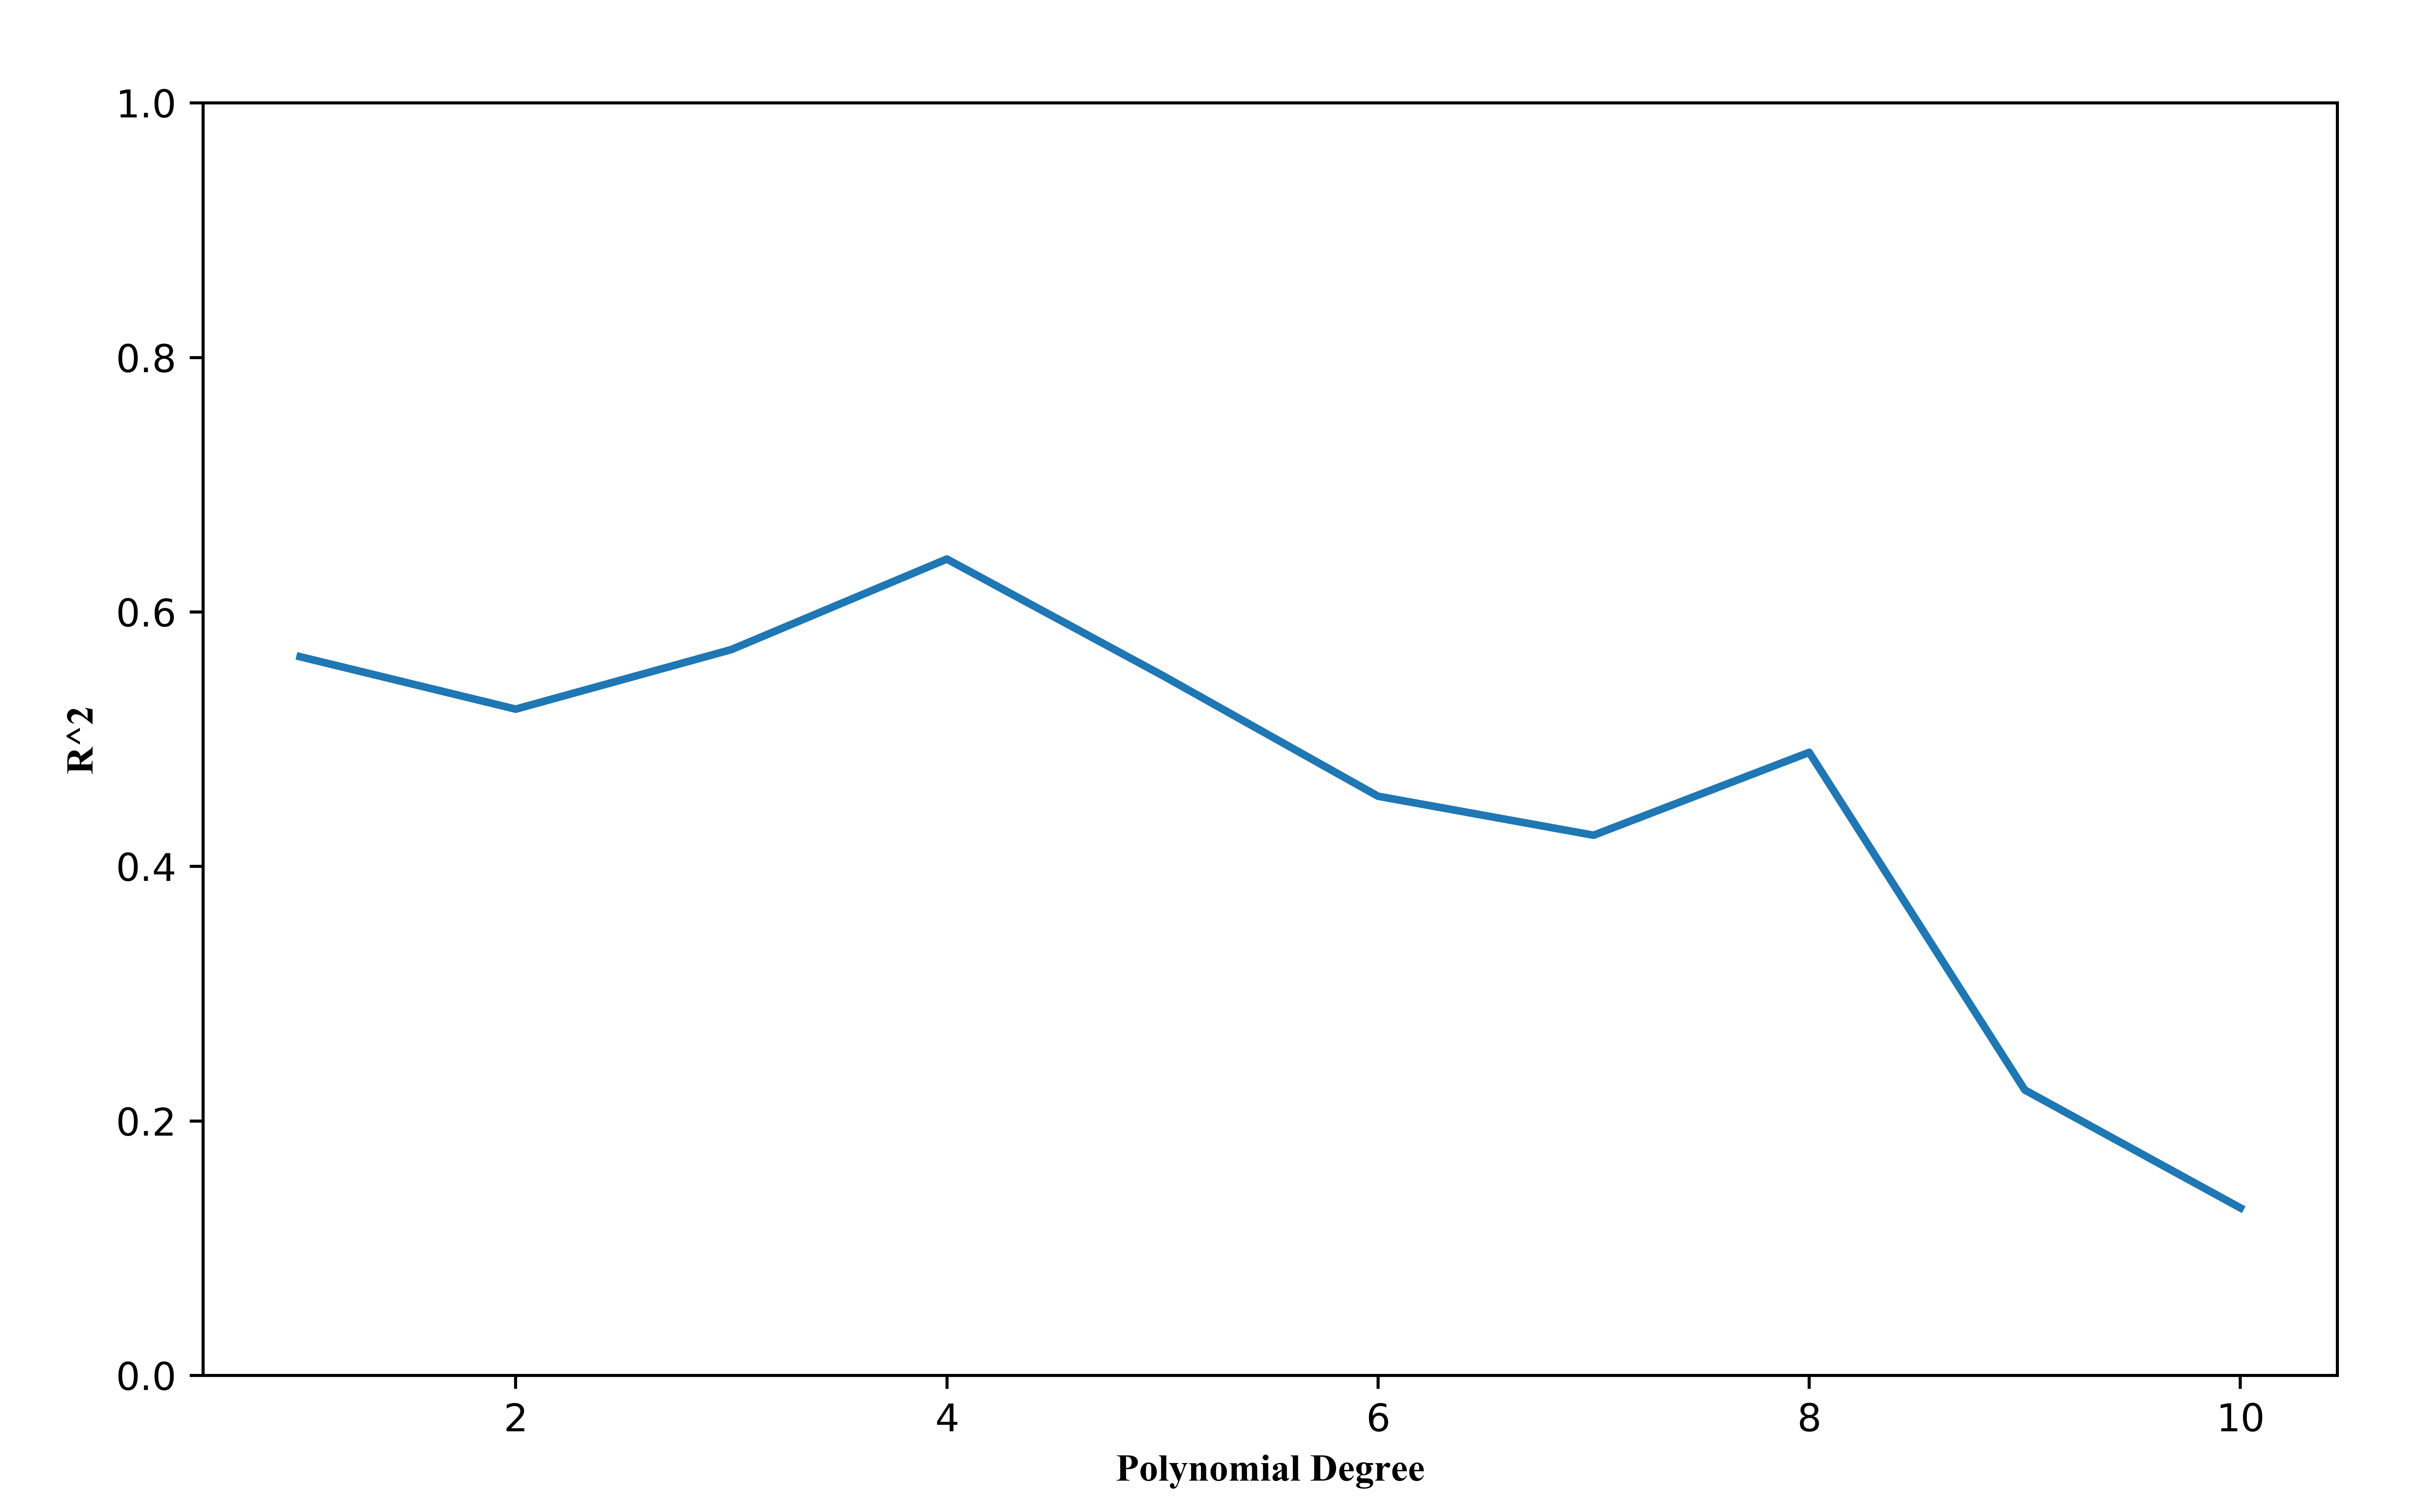
\includegraphics[scale=0.15]{rsquare.png}
\caption{R-squared score of polynomial models with variety of orders when predicting the test data}\label{fig=rsquare.png}
\end{center}
\end{figure}

\noindent 
Based on the Figure \ref{fig=rsquare.png}, polynomial model with order in between two until four will be good candidates. In order to find which order will fits and best to generalize the data points in this particular problem, several graphs are created, as shown in Figure \ref{fig=pol24.png} and Figure \ref{fig=corrrainpeopreg.png}.\\

\begin{figure}
\begin{center}
\graphicspath{ {./Pict/} }
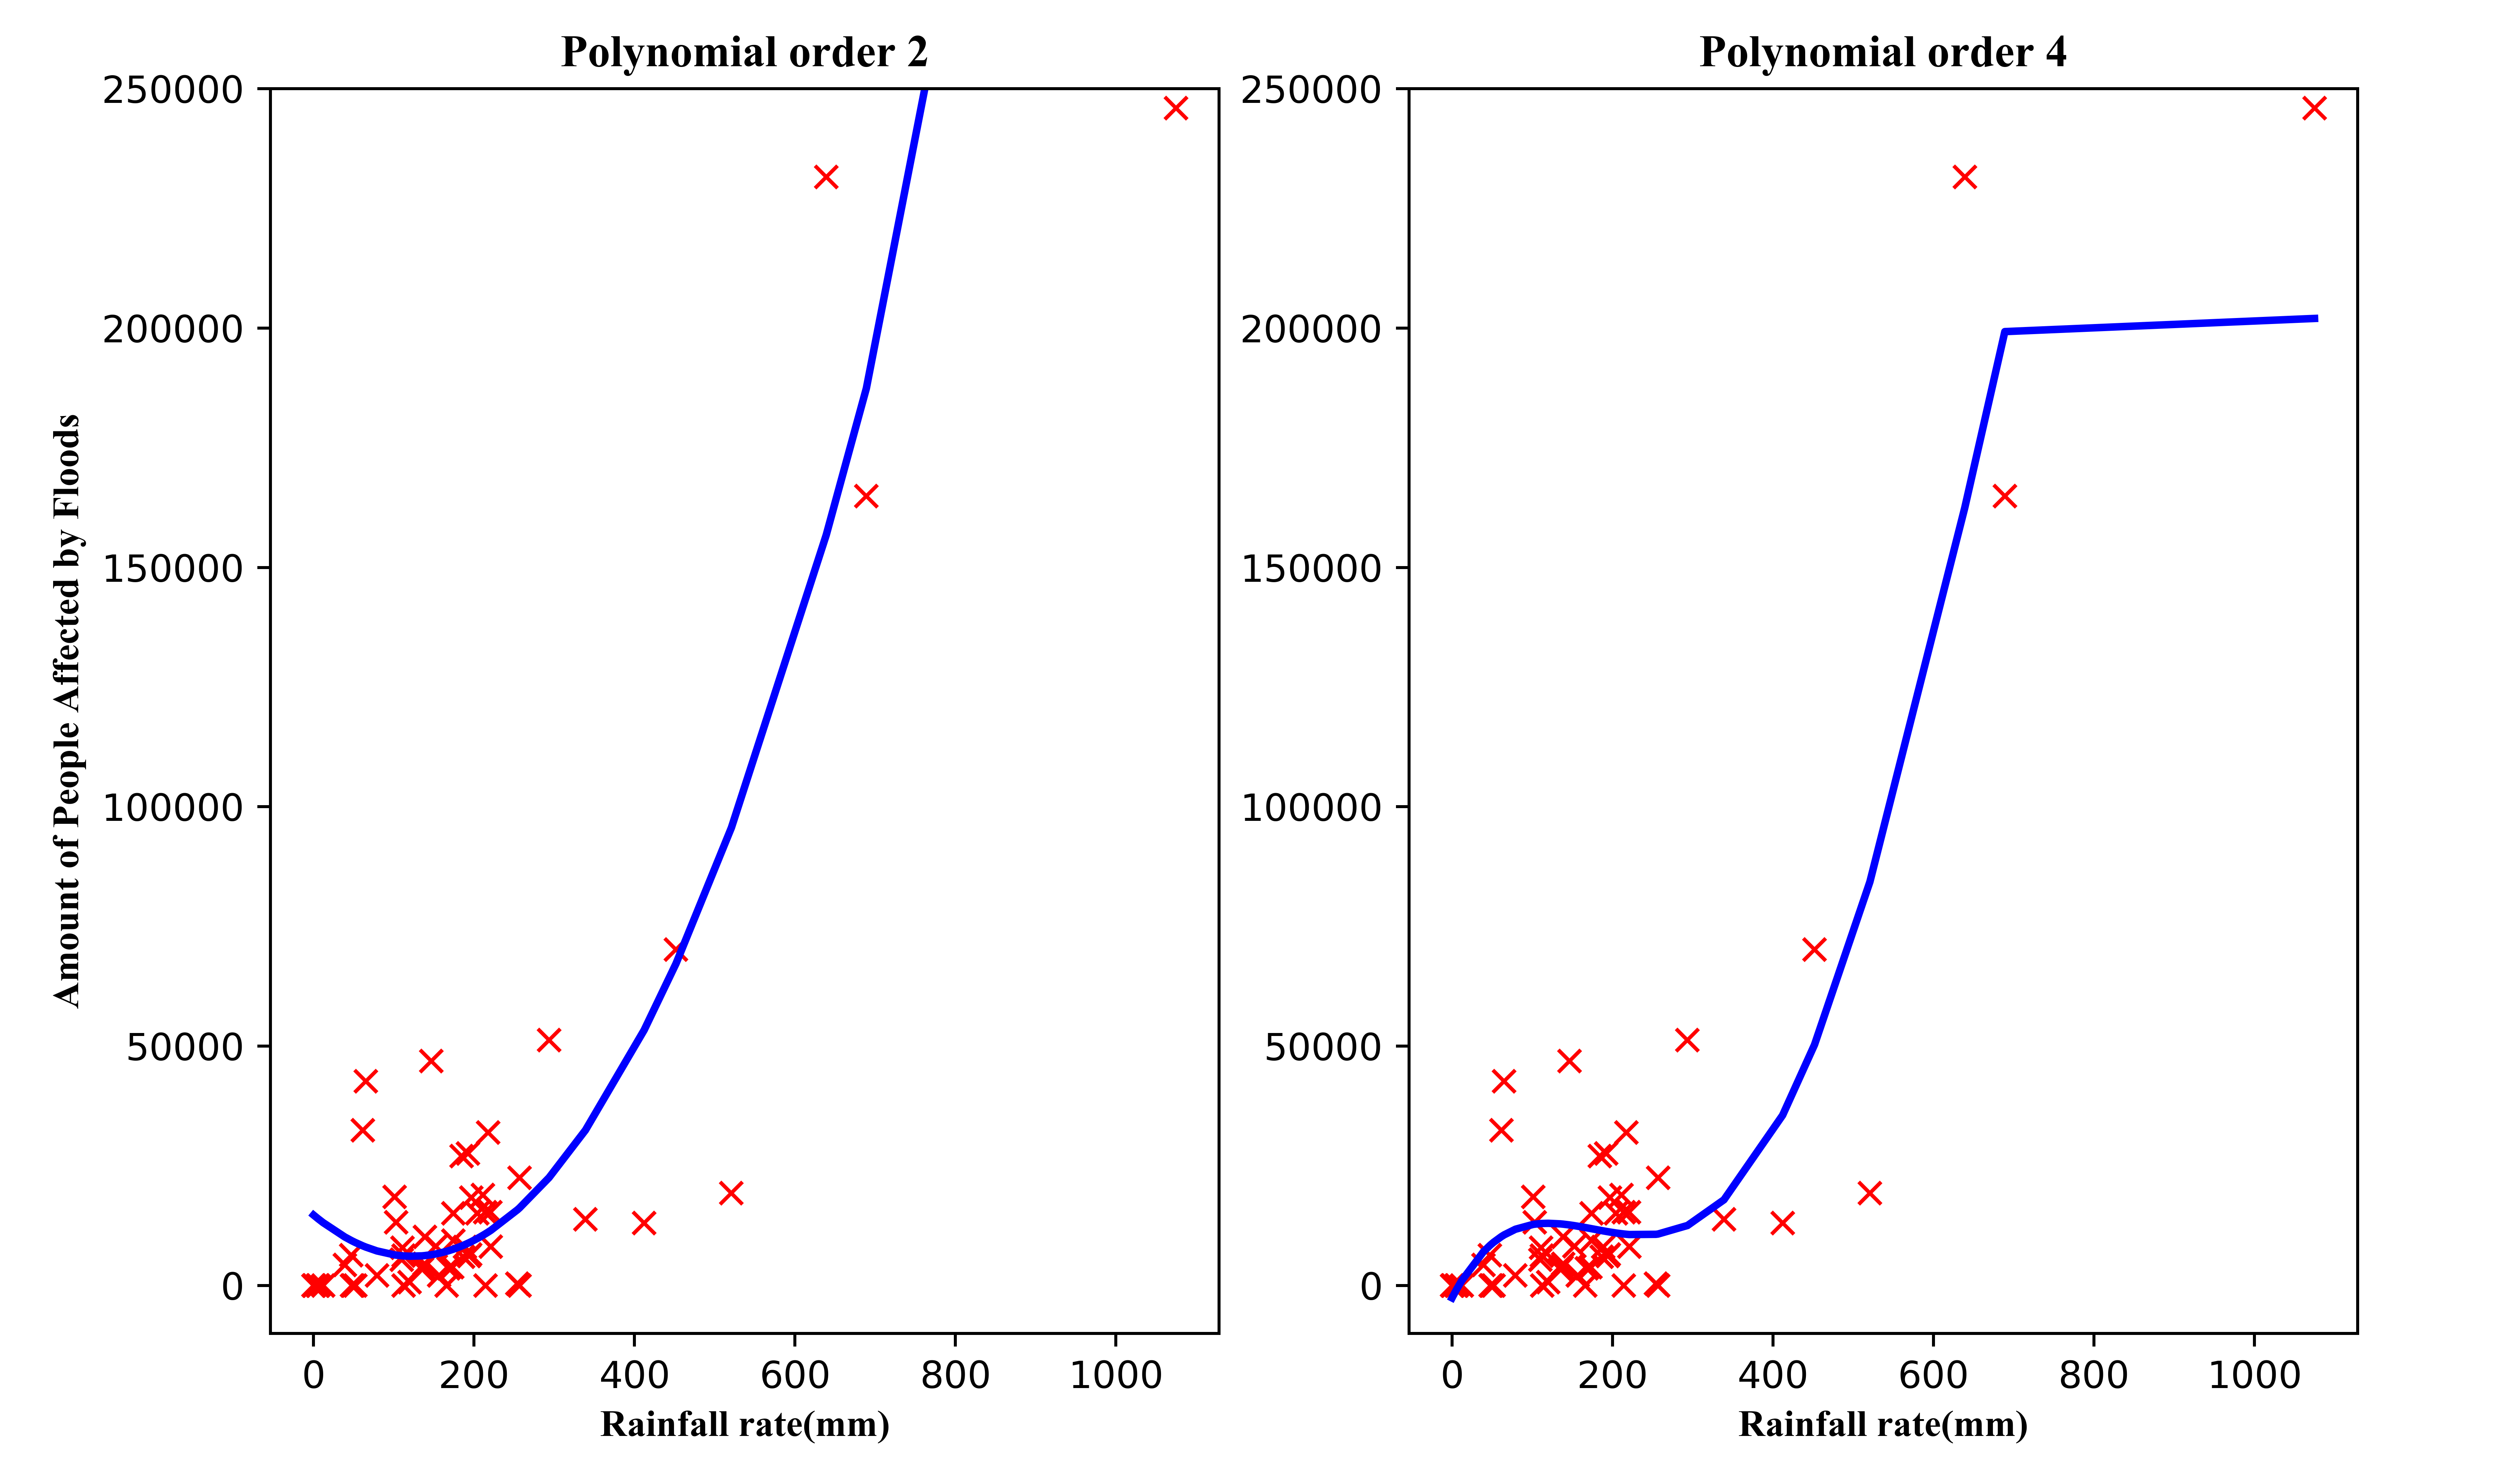
\includegraphics[scale=0.15]{pol24.png}
\caption{Comparison between polynomial regression models with order=2 and order=4}\label{fig=pol24.png}
\end{center}
\end{figure}

\noindent 
In Figure \ref{fig=pol24.png}, it can be concluded that polynomial model with order 2 is slightly underfitting the data points, particularly in the lower region of the graphs. Meanwhile, polynomial model with order 4 is shown some signs of overfitting that won't generalize well with the trends in data points. In Figure \ref{fig=corrrainpeopreg.png}, it can be clearly seen that the polynomial model with order of 3 will yield to the best prediction for this particular problem.\\

\begin{figure}
\begin{center}
\graphicspath{ {./Pict/} }
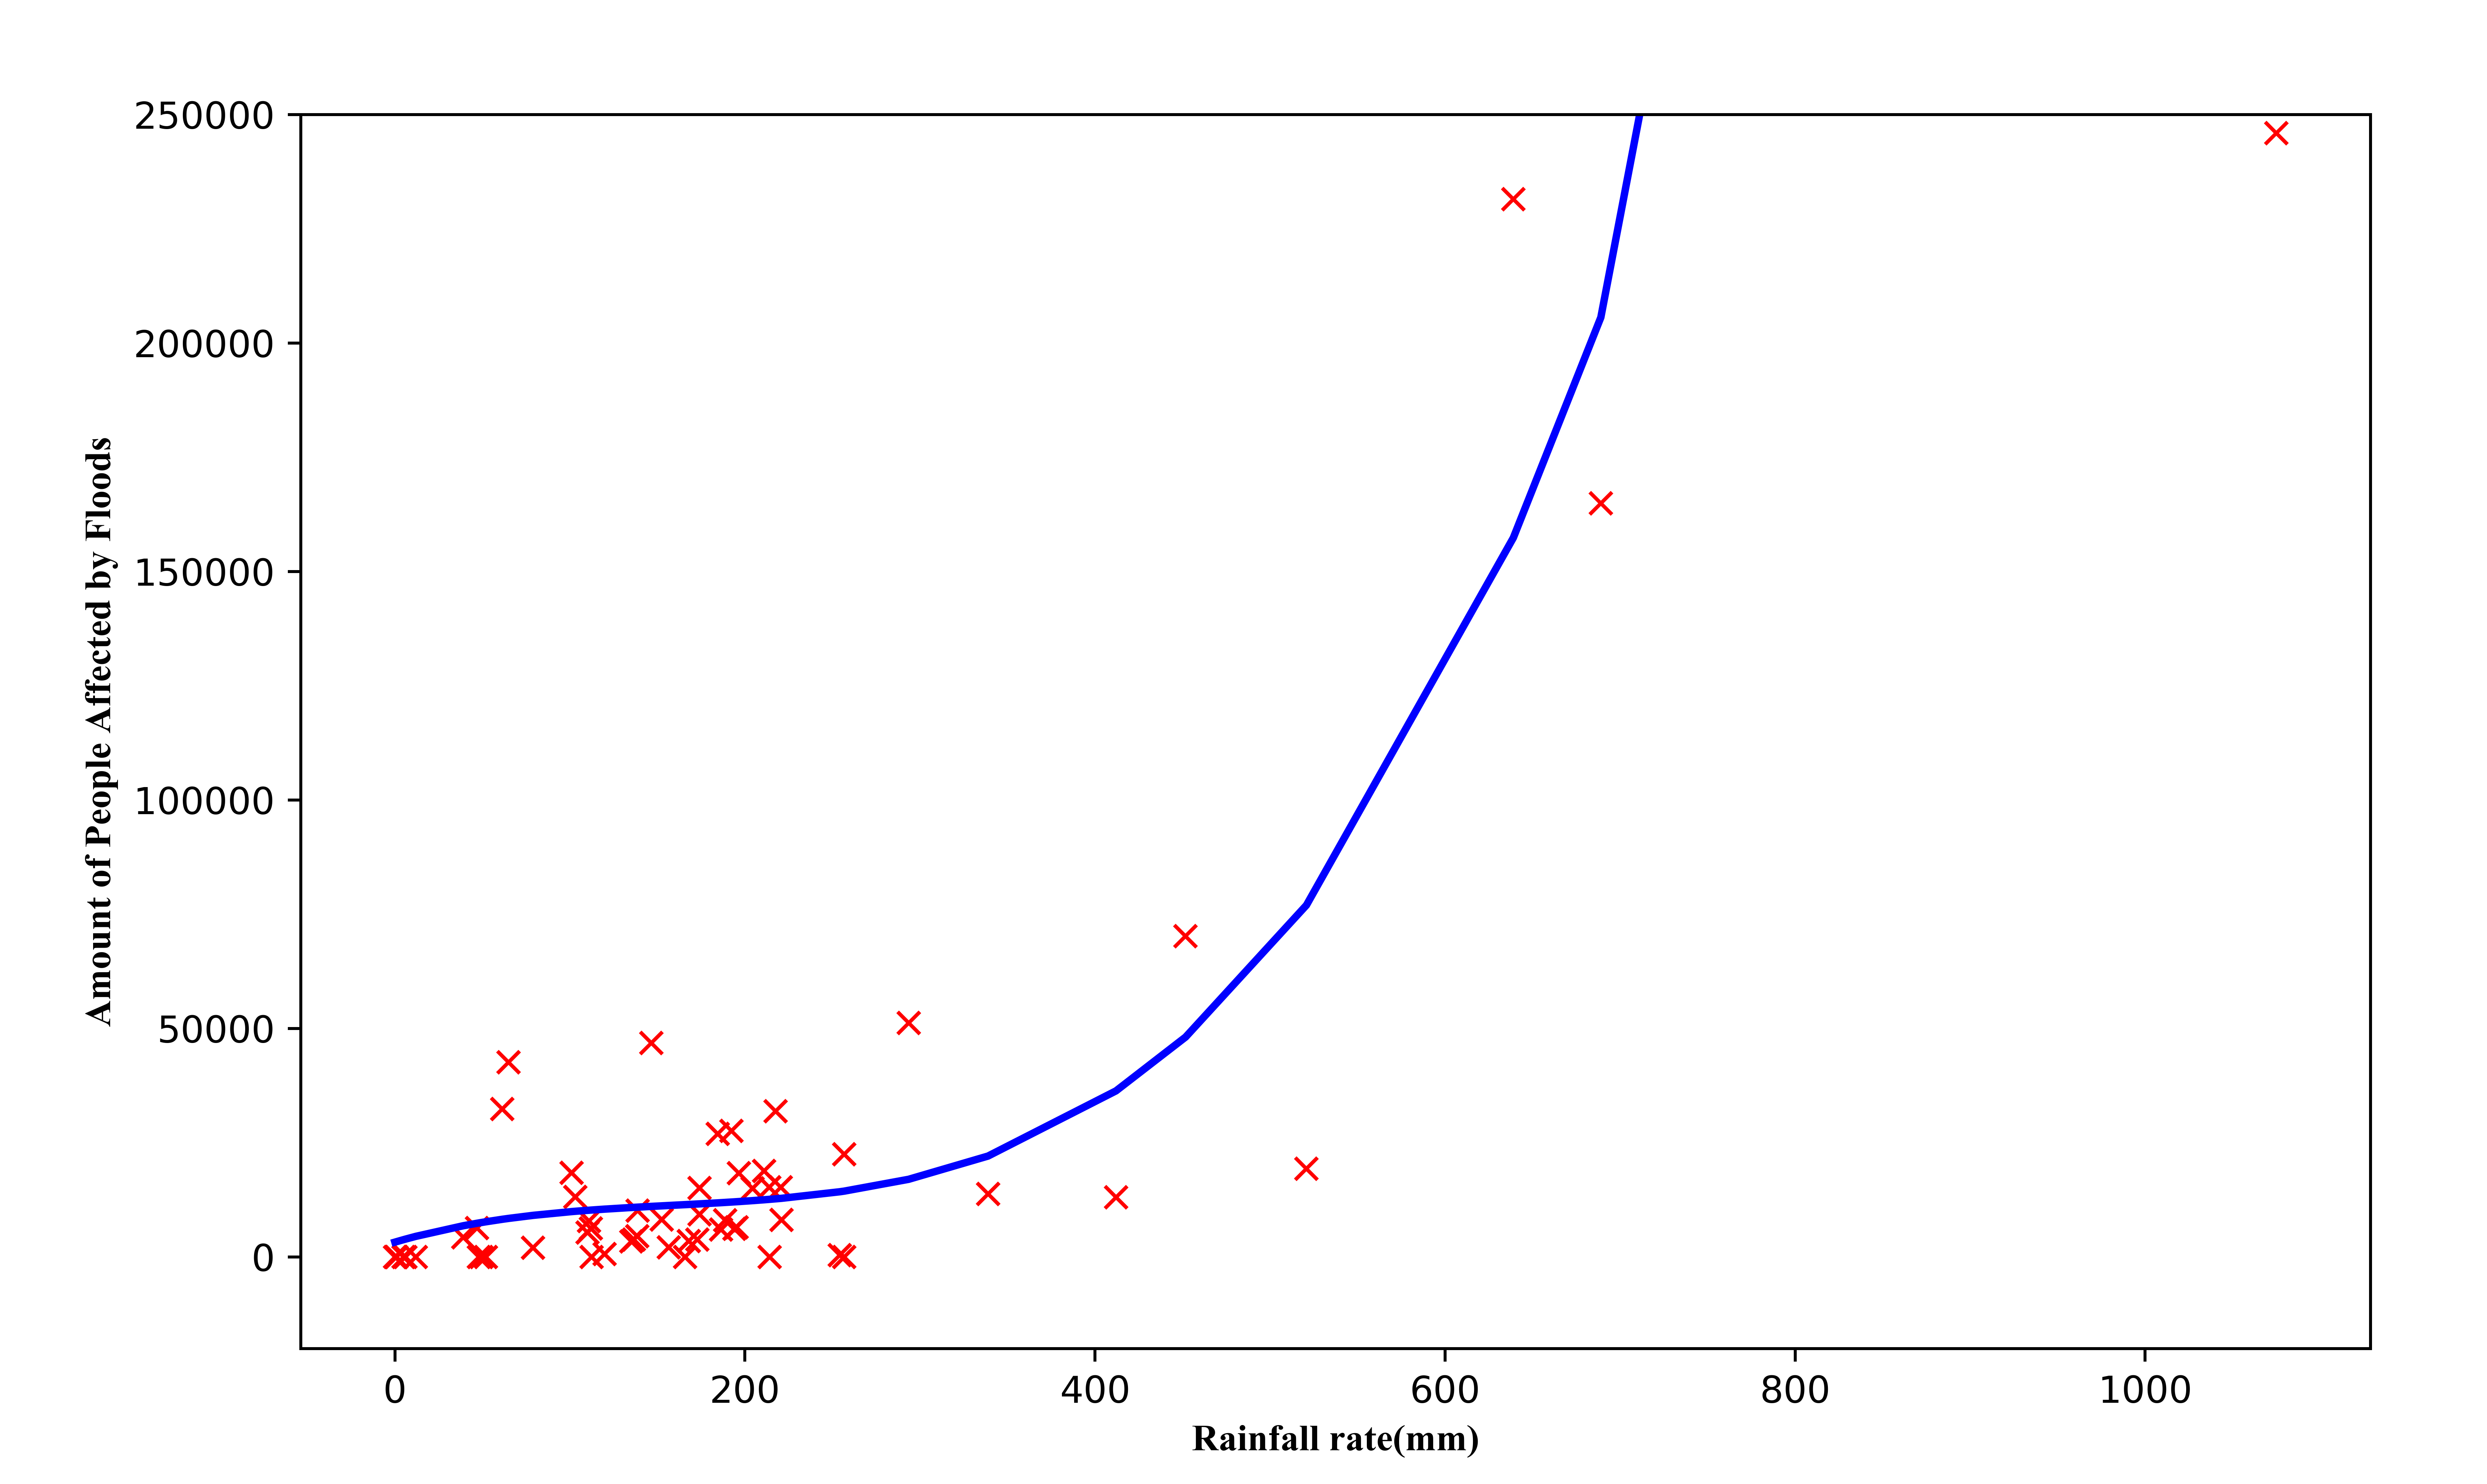
\includegraphics[scale=0.15]{corrrainpeopreg.png}
\caption{Polynomial model with order=3 to estimate the amount of people who will be affected by floods in any given rainfall rate}\label{fig=corrrainpeopreg.png}
\end{center}
\end{figure}
\noindent
With polynomial model with order of 3, now the amount of people who will be affected by floods can be estimated in any given rainfall rate. This would be particularly helpful for the local authorities, the rescue teams, and the medical teams to be prepared once the heavy rainfall pours down the city.


